\documentclass[12pt]{article}
\usepackage[colorlinks=true, linkcolor=blue, breaklinks=true]{hyperref} 
\usepackage{graphicx}
\usepackage{charter,amsmath,amssymb,breakurl}
\usepackage{eulervm}
\usepackage[letterpaper,margin=1in]{geometry}
\usepackage{multicol}
\everymath{\displaystyle}
\author{}\date{Due in class Friday 13 February}
\title{Math 104 Written Assignment 3}\author{}
\begin{document}
\maketitle
\pagestyle{empty}

\begin{center}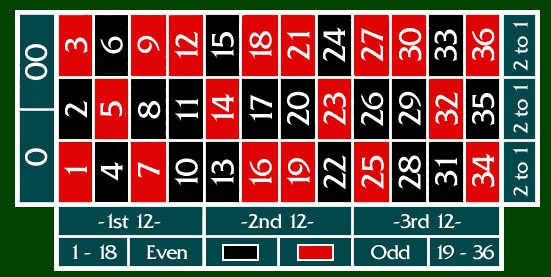
\includegraphics[scale=.3]{RouletteLayout}\end{center}
\begin{enumerate}
\item A {\em corner bet} is a roulette bet on any four numbers that form
a contiguous square on the roulette layout, which is shown above.
For example, a player could make a corner bet on the numbers
$\left\{1,2,4,5\right\}$
\begin{enumerate}
\item Using the formula $\frac{36}{n}-1$ calculate the amount
the casino pays for a winning $\$1$ corner bet.
\item Calcaulte the probabilities of winning and losing a corner bet.
\item Calculate the expectation for a corner bet.
\end{enumerate}

\item A {\em split} is a roulette bet on any two adjoining numbers
on the roulette layout.
For example, a player could make a corner bet on the numbers
$\left\{1,4\right\}$
Another example might be $\left\{1,2\right\}$
\begin{enumerate}
\item Calculate the amount the casino pays for a winning $\$1$ split.
\item Calcaulte the probabilities of winning and losing a split.
\item Calculate the expectation for a split.
\end{enumerate}

\item More generally, calcaluate the expectation on a $\$1$ bet on
$n$~numbers for any $n$. Of course, the $n$~numbers the player can
choose are subject to the rules of roulette, which in turn are determined
by the way the layout is arranged.

\end{enumerate}
\end{document}
